\chapter{Gap-Filling}
\label{app:gap-filling}

Table~\ref{tab:gf_published_replication} records the source-specific methane
gap-filling adaptations removed from the main chapter. Differences in
ecosystem, predictors, measurement period and validation design mean that the
reported source values provide context rather than controlled performance
comparisons \cite{irvin2021,kim2020,zhu2023a}.

\begin{table}[htbp]
\centering
\footnotesize
\begin{tabular}{llcc}
\toprule
Replication & Model & NWFP $R^2$ & Cited $R^2$ \\
\midrule
Irvin et al.\textsuperscript{\dag} & RF & 0.122 & 0.79 \\
(17-site wetland benchmark) & XGBoost & 0.125 & $\approx$0.65--0.67 \\
\midrule
\multirow{2}{*}{\textbf{Zhu et al.\ (UK pasture)}\textsuperscript{\ddag}} & MDS & \textbf{0.055} & $\approx$0.03--0.05 \\
 & RFm & 0.054 & $<0.10$ \\
\midrule
\multirow{5}{*}{Kim et al.\textsuperscript{\P} (wetland/rice paddy)} & MDS & 0.032 & $\approx$0.06--0.71 \\
 & RF & 0.135 & $\approx$0.82--0.97 \\
 & RF + PCA7 & 0.103 & $\approx$0.76--0.96 \\
 & ANN & 0.139 & $\approx$0.64--0.94 \\
 & SVM & 0.057 & $\approx$0.33--0.82 \\
\bottomrule
\end{tabular}
\caption{
    Contextual adaptations of published methane gap-filling baselines.
NWFP values are averaged equally across the towers included by each adaptation;
cited values are those reported by the corresponding source. Only Zhu et al. is comparable to the NWFP pasture ecosystem.
}
\label{tab:gf_published_replication}
\end{table}

\begin{table}[htbp]
\centering
\footnotesize
\begin{tabular*}{0.72\textwidth}{@{\extracolsep{\fill}}lrr@{}}
\toprule
Model or experiment & RMSE & MAE \\
\midrule
Training-set mean & 134.39 & 53.01 \\
MDS & 140.58 & 53.67 \\
RF (meteorology features only) & 129.47 & 51.04 \\
MICE & 125.88 & 59.08 \\
HyperImpute & 105.90 & 45.85 \\
RF (additional features) & \textbf{94.14} & 41.11 \\
LightGBM & 97.55 & 43.57 \\
XGBoost & 103.17 & 49.21 \\
SAITS & 105.35 & 44.44 \\
Bidirectional LSTM & 112.41 & 45.67 \\
TabICLv2 & 95.60 & \textbf{40.69} \\
\bottomrule
\end{tabular*}
\caption{Aggregate error metrics for the gap-filling models in
Table~\ref{tab:gf_model_comparison}. Values are equal-weight averages of the
three tower-specific median scores across the common synthetic-gap settings.
RMSE and MAE are reported in
$\mathrm{nmol\,m^{-2}\,s^{-1}}$; lower values are preferable.}
\label{tab:gf_error_metrics_aggregate}
\end{table}

\begin{figure}[p]
\centering
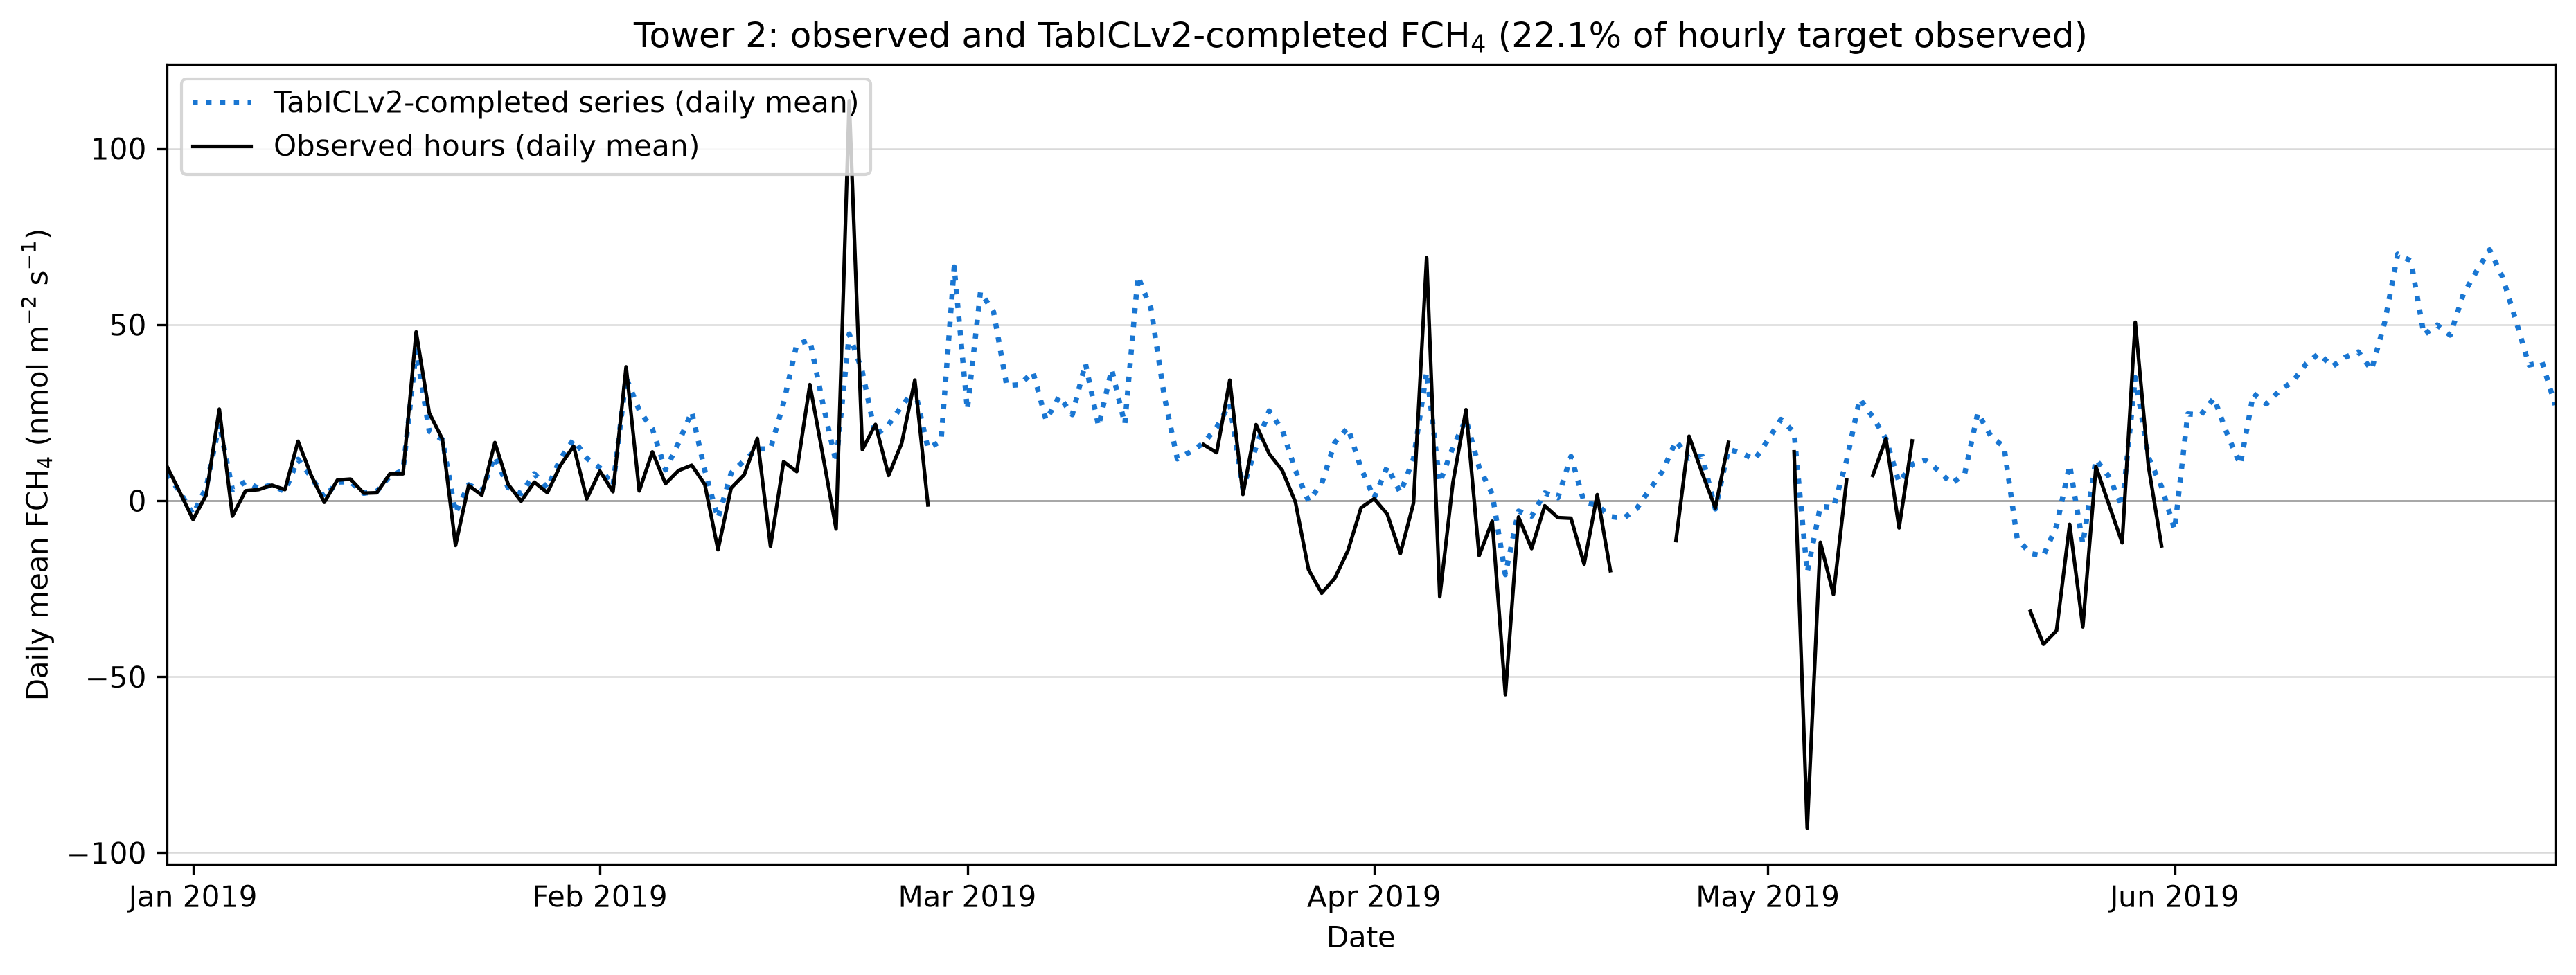
\includegraphics[width=\textwidth]{Figures/ch4_tabiclv2_daily_T2_2019H1.png}
\vspace{0.5em}

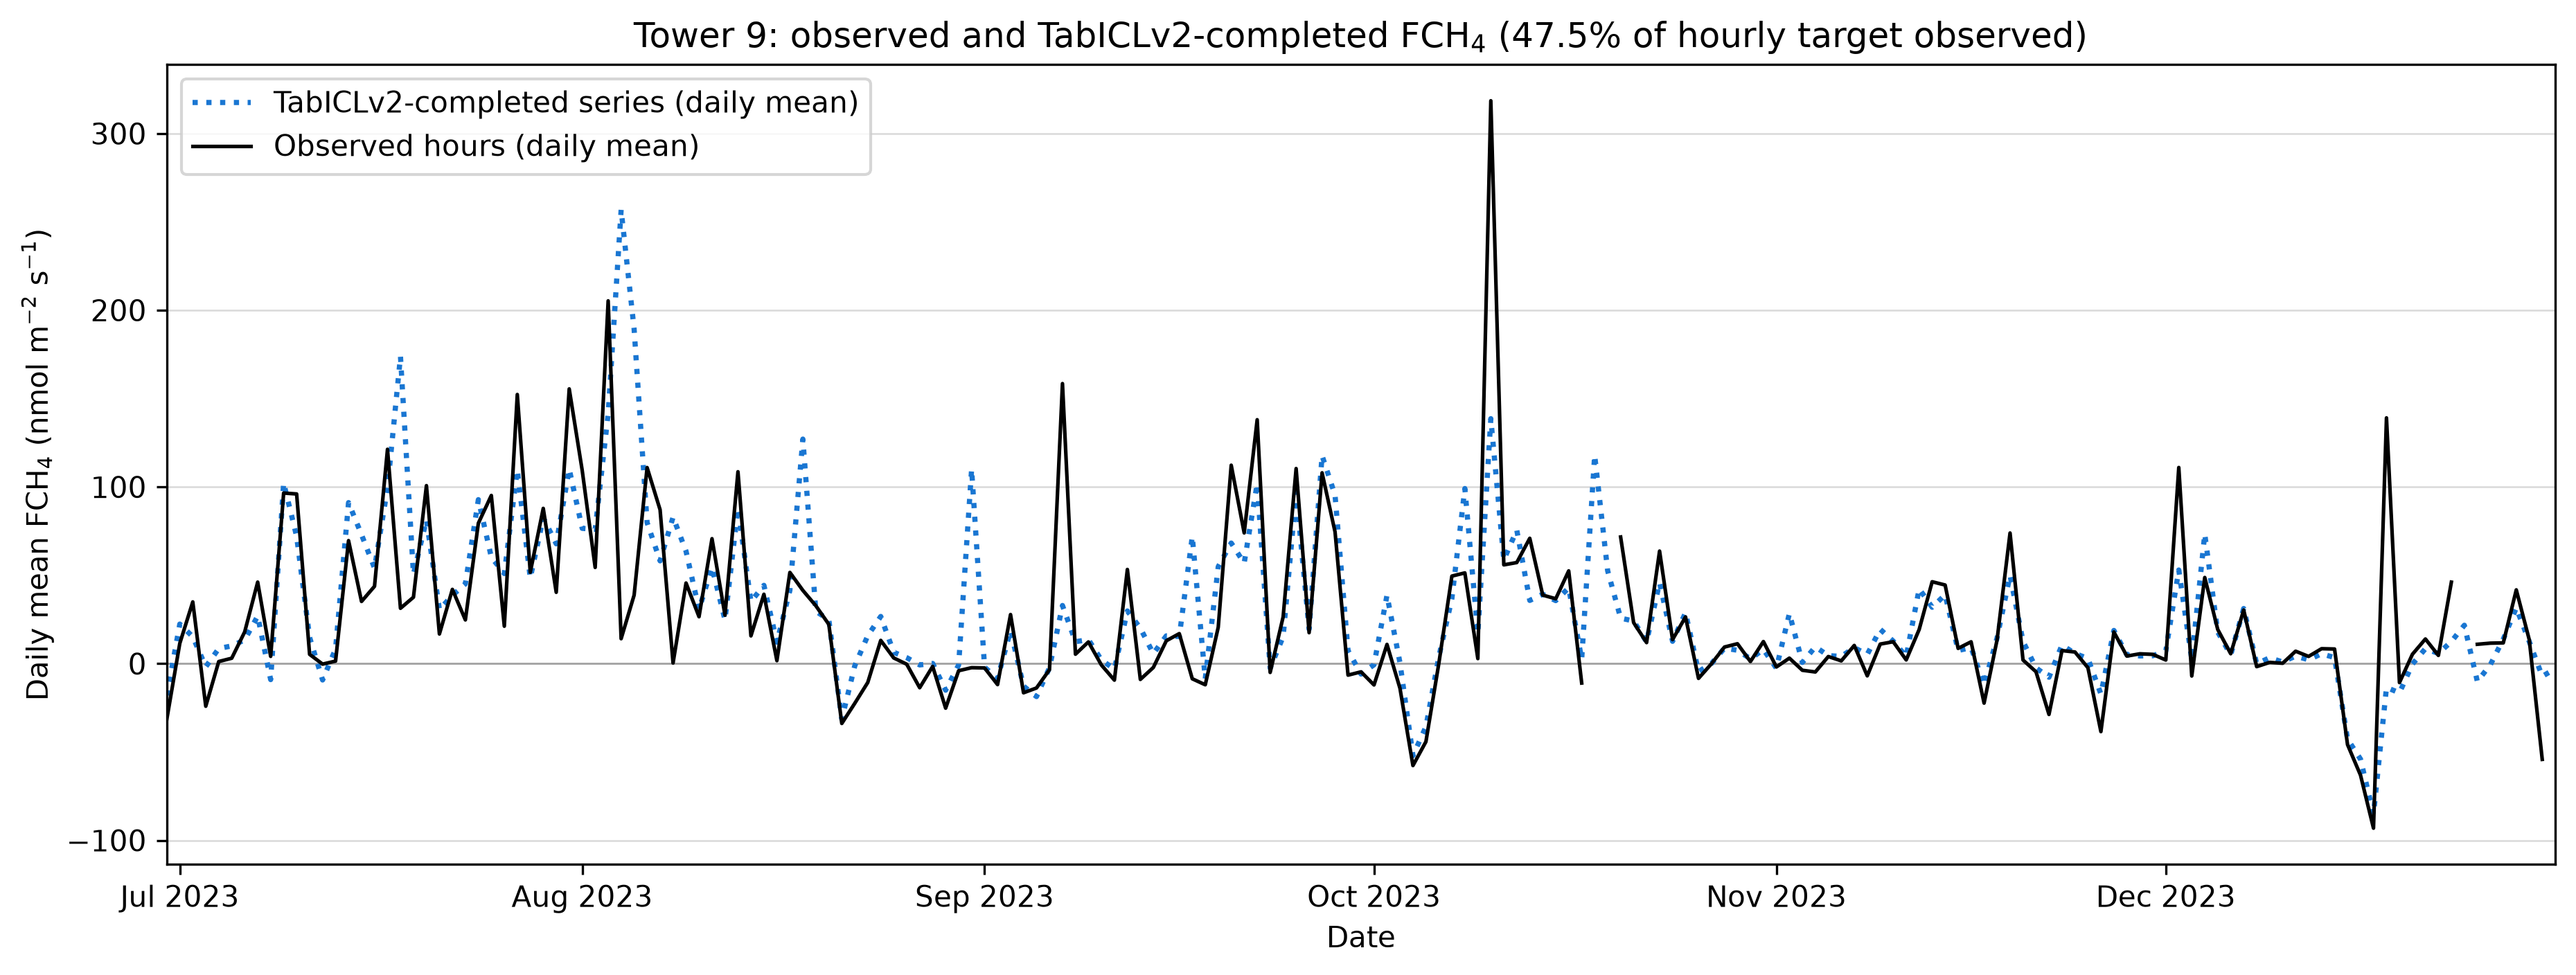
\includegraphics[width=\textwidth]{Figures/ch4_tabiclv2_daily_T9_2023H2.png}
\caption{Daily means from QC-valid observed hours (solid black) and the
TabICLv2-completed series (dotted blue) at T2 during January--June 2019 (top)
and T9 during July--December 2023 (bottom). Hourly target availability was
22.1\% at T2 and 47.5\% at T9. The completed series preserves observations and
fills missing hours with TabICLv2 estimates; the panels are reconstruction
diagnostics rather than held-out validation. The corresponding T4 example is
shown in Figure~\ref{fig:gf_t4_reconstruction}.}
\label{fig:app_gf_tabicl_daily_t2_t9}
\end{figure}

\begin{figure}[p]
\centering
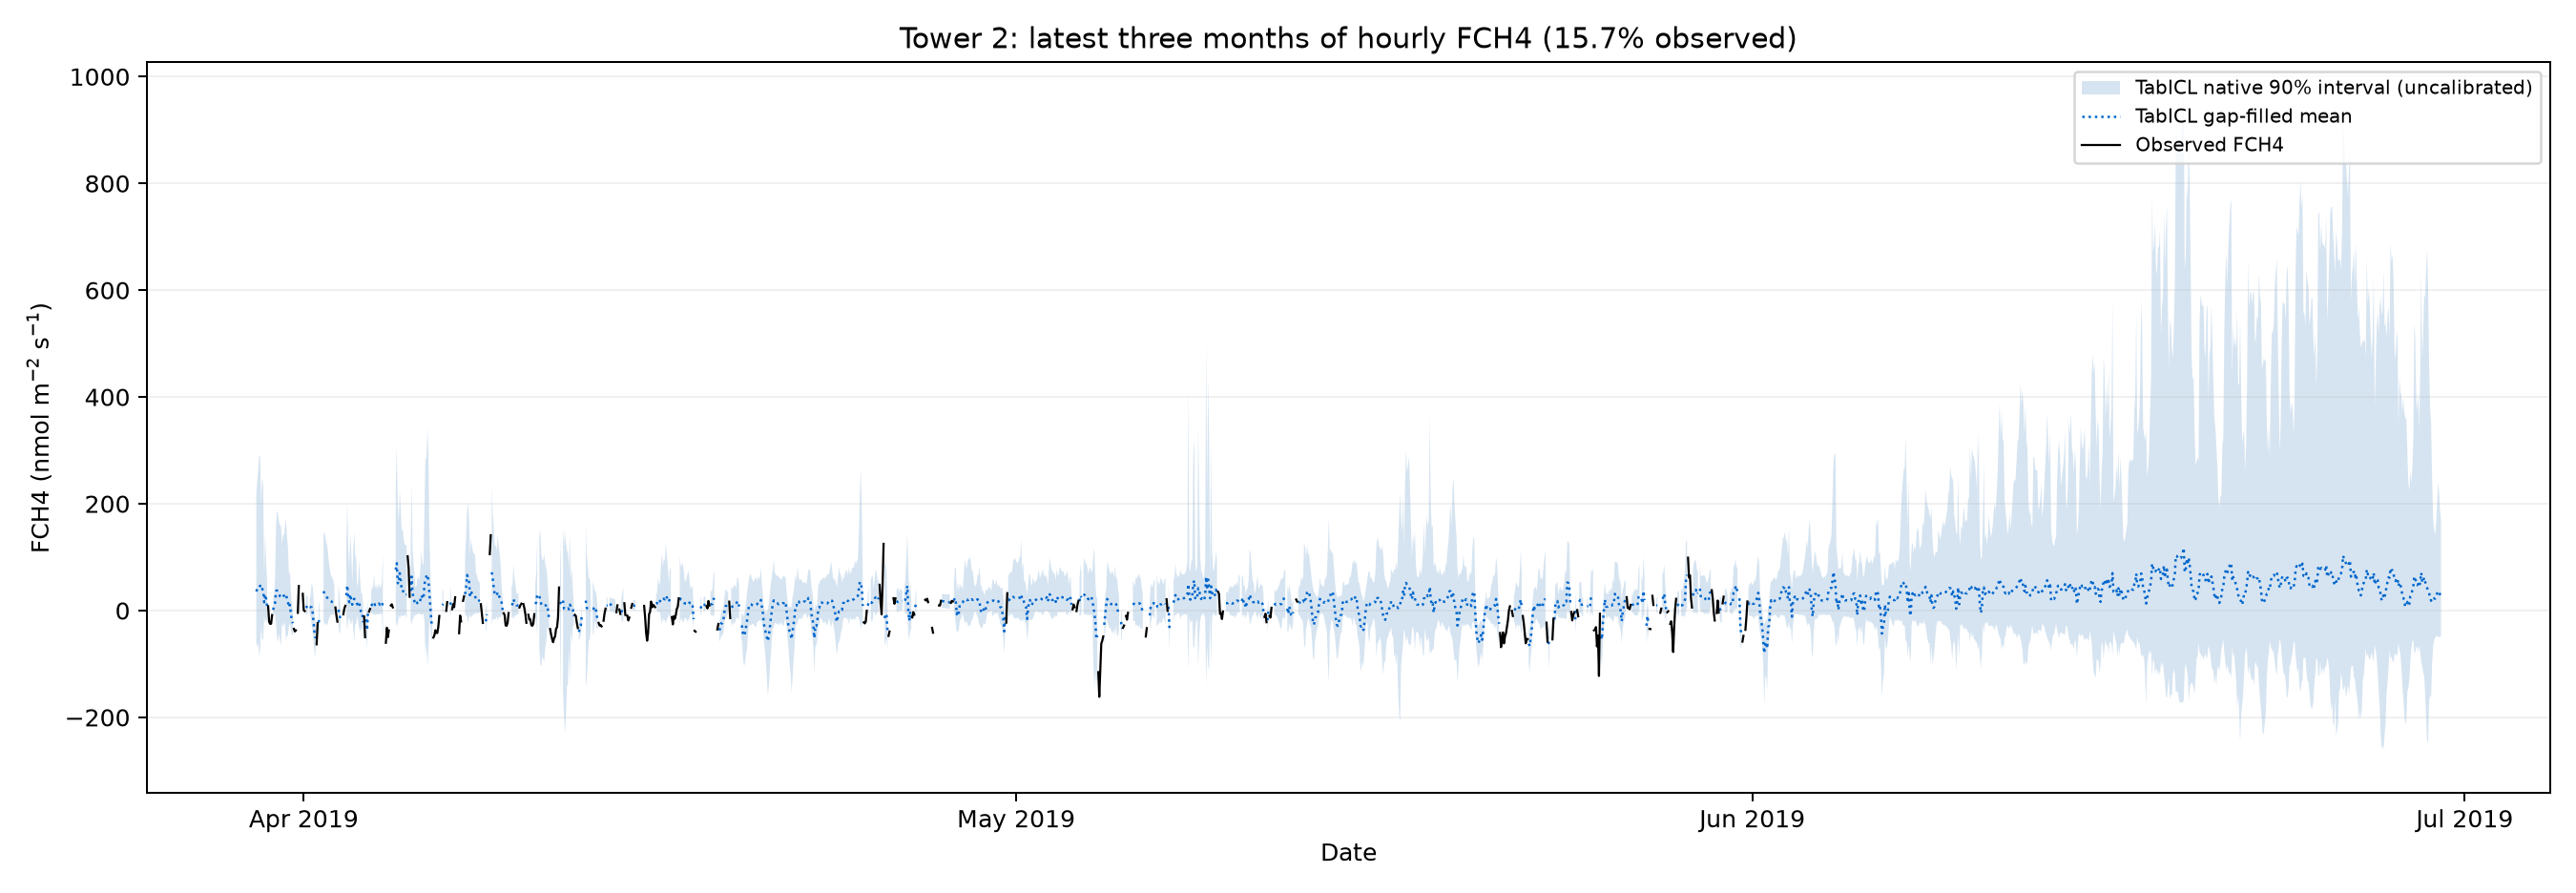
\includegraphics[width=\textwidth]{Figures/ch4_latest_tabicl_uq_hourly_T2_3month_example.png}
\vspace{0.5em}

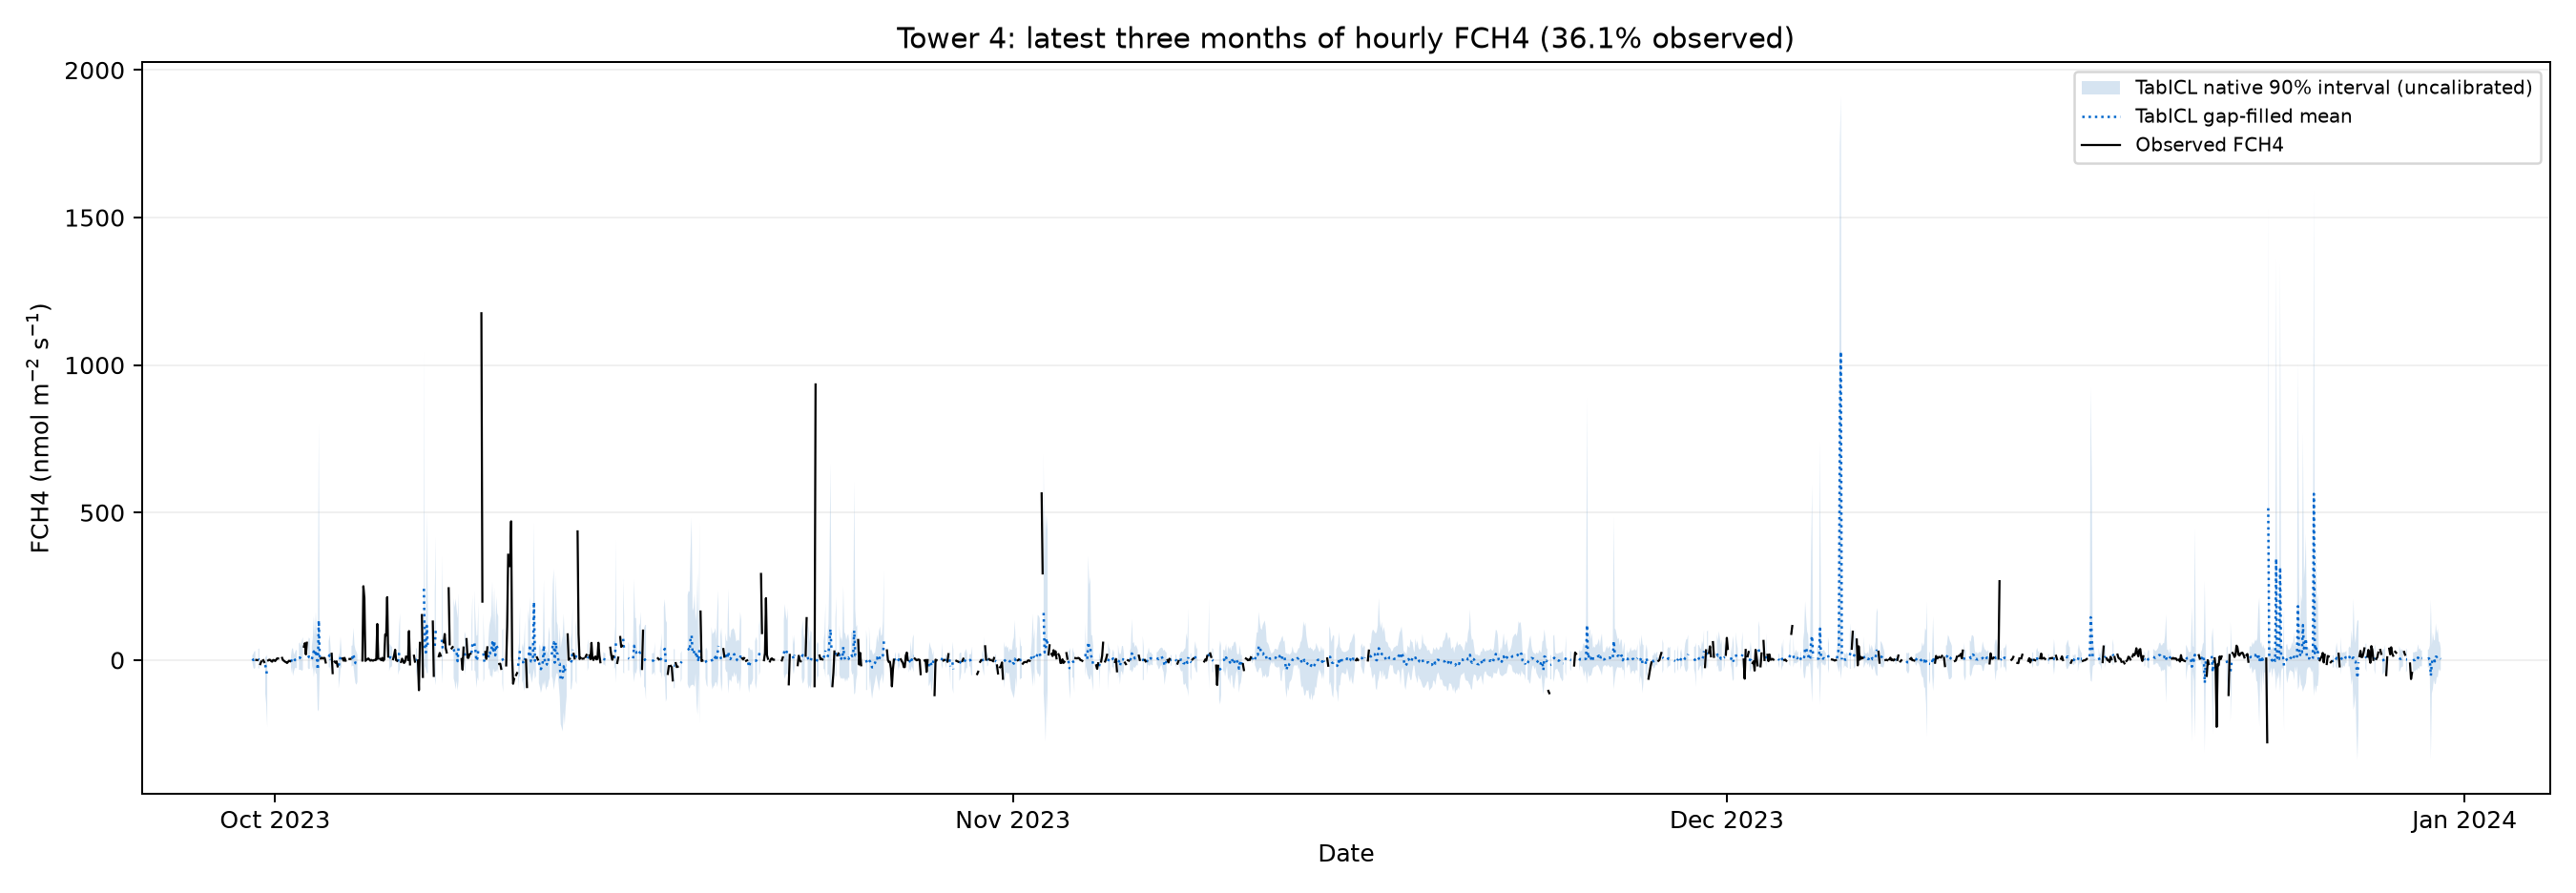
\includegraphics[width=\textwidth]{Figures/ch4_latest_tabicl_uq_hourly_T4_3month_example.png}
\caption{Three-month examples of hourly FCH\textsubscript{4} reconstruction
and native uncertainty for T2 (top) and T4 (bottom). Black lines show QC-valid
observations, dotted blue lines show the TabICLv2 gap-filled mean, and shaded
regions show the uncalibrated native 90\% interval. Each tower uses its latest
available three-month window and its own vertical scale.}
\label{fig:app_gf_tabicl_t2_t4}
\end{figure}

\FloatBarrier

